\documentclass[tikz,border=10pt]{standalone}
\usepackage{tikz}
\usepackage{amsmath,amssymb}
\usetikzlibrary{positioning, arrows.meta, calc, fit, backgrounds, shapes.geometric}

\begin{document}
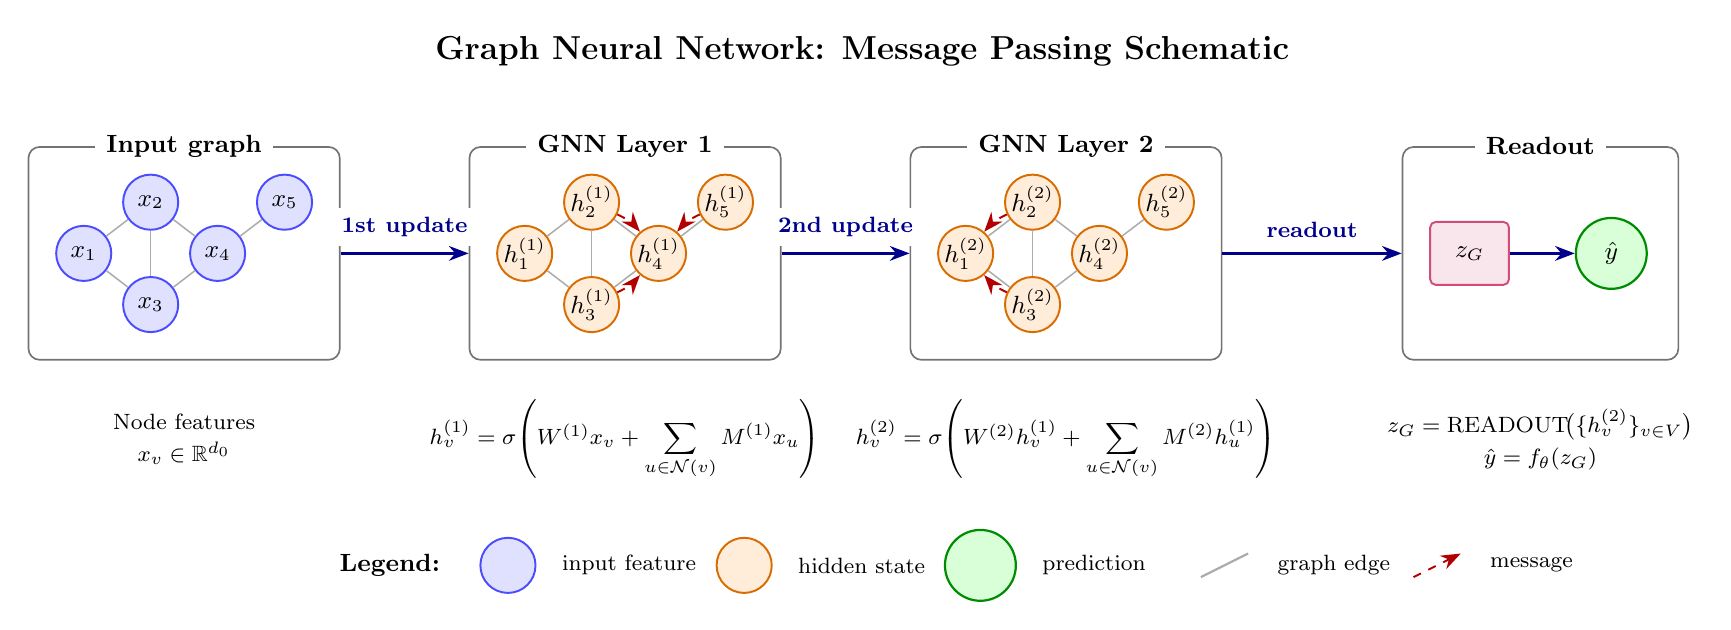
\begin{tikzpicture}[
    >={Stealth[length=2.5mm]},
    inputnode/.style ={circle, draw=blue!70,        fill=blue!12,    line width=0.7pt, minimum size=7mm, inner sep=0pt, font=\small},
    hiddennode/.style={circle, draw=orange!85!black, fill=orange!15, line width=0.7pt, minimum size=7mm, inner sep=0pt, font=\small},
    outnode/.style   ={circle, draw=green!55!black,  fill=green!15,  line width=0.8pt, minimum size=9mm, inner sep=0pt, font=\small},
    poolnode/.style  ={rectangle, rounded corners=2pt, draw=purple!70, fill=purple!10,
                       line width=0.7pt, minimum width=10mm, minimum height=8mm, font=\small},
    edge/.style={-, gray!65, line width=0.55pt},
    msg/.style ={->, red!70!black, line width=0.7pt, dashed},
    flow/.style={->, thick, blue!55!black, line width=1.0pt},
    layerbox/.style={draw=black!55, line width=0.6pt, rounded corners=4pt,
                     inner sep=10pt},
    boxtitle/.style={font=\bfseries\small, fill=white, inner xsep=4pt, inner ysep=1pt},
    flowlabel/.style={font=\footnotesize\bfseries, blue!55!black, fill=white, inner xsep=2pt},
    eqcaption/.style={font=\footnotesize, align=center}
]

% =====================================================
% Node coordinates inside one layer (reused for all 3)
% Compact layout: a (left), b (top-mid), c (bot-mid),
% d (right-mid), e (top-right)
% =====================================================
\def\layout{
    \coordinate (na) at (0.00, 0.00);
    \coordinate (nb) at (0.85, 0.65);
    \coordinate (nc) at (0.85,-0.65);
    \coordinate (nd) at (1.70, 0.00);
    \coordinate (ne) at (2.55, 0.65);
}

% =====================================================
% Helper: draw the 5-node graph at the current scope
% style = nodename style
% prefix = unique node-name prefix for cross-references
% labels = which symbol in each node (#1..#5)
% =====================================================

% --- Input layer (L0) at x = 0
\begin{scope}[shift={(0,0)}, local bounding box=L0graph]
    \layout
    \node[inputnode] (a0) at (na) {$x_1$};
    \node[inputnode] (b0) at (nb) {$x_2$};
    \node[inputnode] (c0) at (nc) {$x_3$};
    \node[inputnode] (d0) at (nd) {$x_4$};
    \node[inputnode] (e0) at (ne) {$x_5$};
    \draw[edge] (a0)--(b0); \draw[edge] (a0)--(c0);
    \draw[edge] (b0)--(c0); \draw[edge] (b0)--(d0);
    \draw[edge] (c0)--(d0); \draw[edge] (d0)--(e0);
\end{scope}
\node[layerbox, fit=(L0graph)] (box0) {};
\node[boxtitle] at (box0.north) {Input graph};

% --- Layer 1 at x = 5.6
\begin{scope}[shift={(5.6,0)}, local bounding box=L1graph]
    \layout
    \node[hiddennode] (a1) at (na) {$h^{(1)}_1$};
    \node[hiddennode] (b1) at (nb) {$h^{(1)}_2$};
    \node[hiddennode] (c1) at (nc) {$h^{(1)}_3$};
    \node[hiddennode] (d1) at (nd) {$h^{(1)}_4$};
    \node[hiddennode] (e1) at (ne) {$h^{(1)}_5$};
    \draw[edge] (a1)--(b1); \draw[edge] (a1)--(c1);
    \draw[edge] (b1)--(c1); \draw[edge] (b1)--(d1);
    \draw[edge] (c1)--(d1); \draw[edge] (d1)--(e1);
    % Highlight aggregation at d1
    \draw[msg] (b1) to[bend left=12]  (d1);
    \draw[msg] (c1) to[bend right=12] (d1);
    \draw[msg] (e1) to[bend right=12] (d1);
\end{scope}
\node[layerbox, fit=(L1graph)] (box1) {};
\node[boxtitle] at (box1.north) {GNN Layer 1};

% --- Layer 2 at x = 11.2
\begin{scope}[shift={(11.2,0)}, local bounding box=L2graph]
    \layout
    \node[hiddennode] (a2) at (na) {$h^{(2)}_1$};
    \node[hiddennode] (b2) at (nb) {$h^{(2)}_2$};
    \node[hiddennode] (c2) at (nc) {$h^{(2)}_3$};
    \node[hiddennode] (d2) at (nd) {$h^{(2)}_4$};
    \node[hiddennode] (e2) at (ne) {$h^{(2)}_5$};
    \draw[edge] (a2)--(b2); \draw[edge] (a2)--(c2);
    \draw[edge] (b2)--(c2); \draw[edge] (b2)--(d2);
    \draw[edge] (c2)--(d2); \draw[edge] (d2)--(e2);
    % Highlight aggregation at a2 (different node than layer 1)
    \draw[msg] (b2) to[bend right=12] (a2);
    \draw[msg] (c2) to[bend left=12]  (a2);
\end{scope}
\node[layerbox, fit=(L2graph)] (box2) {};
\node[boxtitle] at (box2.north) {GNN Layer 2};

% --- Readout at x = 17.6 (extra gap so 'readout' label has breathing room)
\begin{scope}[shift={(17.6,0)}, local bounding box=L3graph]
    \node[poolnode] (pool) at (0.0,0.0)  {$z_G$};
    \node[outnode]  (out)  at (1.8,0.0)  {$\hat{y}$};
    \draw[flow] (pool) -- (out);
    % anchors to match the height of the graph boxes (y in [-1, 1])
    \coordinate (anchor)  at (-0.5,-1.0);
    \coordinate (anchor2) at ( 2.3, 1.0);
\end{scope}
\node[layerbox, fit=(L3graph) (anchor) (anchor2)] (box3) {};
\node[boxtitle] at (box3.north) {Readout};

% =====================================================
% Inter-box arrows (live in clean gaps between boxes)
% =====================================================
\draw[flow] (box0.east) -- (box1.west)
    node[midway, above=2pt, flowlabel] {1st update};
\draw[flow] (box1.east) -- (box2.west)
    node[midway, above=2pt, flowlabel] {2nd update};
\draw[flow] (box2.east) -- (box3.west)
    node[midway, above=2pt, flowlabel] {readout};

% =====================================================
% Equation captions (own row, well below boxes)
% =====================================================
\def\eqyshift{-1.0cm}
\node[eqcaption] at ($(box0.south) + (0,\eqyshift)$)
    {Node features\\[2pt] $x_v \in \mathbb{R}^{d_0}$};

\node[eqcaption] at ($(box1.south) + (0,\eqyshift)$)
    {$h^{(1)}_v = \sigma\!\left(W^{(1)} x_v + \displaystyle\sum_{u\in\mathcal{N}(v)} M^{(1)} x_u\right)$};

\node[eqcaption] at ($(box2.south) + (0,\eqyshift)$)
    {$h^{(2)}_v = \sigma\!\left(W^{(2)} h^{(1)}_v + \displaystyle\sum_{u\in\mathcal{N}(v)} M^{(2)} h^{(1)}_u\right)$};

\node[eqcaption] at ($(box3.south) + (0,\eqyshift)$)
    {$z_G = \mathrm{READOUT}\!\bigl(\{h^{(2)}_v\}_{v\in V}\bigr)$\\[2pt]
     $\hat{y} = f_\theta(z_G)$};

% =====================================================
% Title (top, centered over the full row)
% =====================================================
\node[font=\bfseries\large] at ($(box0.north)!0.5!(box3.north) + (0,1.2)$)
    {Graph Neural Network: Message Passing Schematic};

% =====================================================
% Legend (clean horizontal row at bottom, centered)
% =====================================================
\node (legendanchor) at ($(box0.south)!0.5!(box3.south) + (0,-2.6)$) {};
\begin{scope}[shift={(legendanchor)}]
    \node[font=\bfseries\small] (lg0) at (-6.0,0)  {Legend:};
    \node[inputnode]  (lg1) at (-4.5,0) {};
    \node[right=2mm of lg1, font=\footnotesize] (lglab1) {input feature};
    \node[hiddennode] (lg2) at (-1.5,0) {};
    \node[right=2mm of lg2, font=\footnotesize] (lglab2) {hidden state};
    \node[outnode]    (lg3) at (1.5,0) {};
    \node[right=2mm of lg3, font=\footnotesize] (lglab3) {prediction};
    \draw[edge, line width=0.8pt] (4.3,-0.15) -- (4.9,0.15);
    \node[right=2mm, font=\footnotesize] at (4.95,0) {graph edge};
    \draw[msg] (7.0,-0.15) -- (7.6,0.15);
    \node[right=2mm, font=\footnotesize] at (7.65,0) {message};
\end{scope}

\end{tikzpicture}
\end{document}
